\documentclass[10pt]{article}
\usepackage{graphicx}
\begin{document}
\title{SmartBalancer}
\author{Raghav Sethi and Nevin Li}
\date{}
\maketitle

\section{Introduction}

\paragraph{} Data centers today, especially multi-tenant cloud environments, run a wide variety of workloads that are constantly changing over time. Software-Defined Networking (SDN) simplifies the datacenter network management process by allowing for programmatic network-wide control. SDN programmers can express complex dynamic policies for routing, load balancing, access control and traffic engineering by leveraging increasingly sophisticated controller platforms like Pyretic\cite{Pyretic} and Onix\cite{Onix}. Load-balancers are an integral part of such multi-tenant cloud deployments, and public cloud providers have invested heavily into designing efficient, scalable systems for this purpose\cite{Ananta}. To optimize SDN-based load balancer performance, programmers use queries for network status and load information (from switches) and route traffic appropriately. There is, however, an opportunity to significantly improve load-balancing performance by leveraging load information available only at the host, i.e. metrics like CPU/memory utilization, process liveness etc. This would give programmers greater visibility into the performance of applications running across individual hosts and would enable the development of load-balancers that can reduce application latency and react to host conditions (which may change rapidly in a multi-tenant scenario).

\paragraph{} In this paper, we make the following contributions:
\begin{enumerate}
\item We describe the design of a low-impact monitoring tool designed to run on end-hosts that collects and communicates metrics like CPU and memory utilization, process liveness etc. to the controller.
\item We discuss the design of SmartBalancer, a Pyretic-based controller application that collects host load information and distributes traffic appropriately
\item We show that SmartBalancer can also be used to dynamically spin up new hosts to deal with excessive incoming traffic, and route traffic to them.
\end{enumerate}


\paragraph{} The rest of the paper is structured as follows. Section 2\ref{sec:related} discusses how this work relates to several other similar systems. Section 3\ref{sec:design} describes the design of the monitoring utility and controller application that comprise SmartBalancer. Section 4\ref{sec:evaluation} shows some preliminary results.

\section{Related Work}
\label{sec:related}

\paragraph{} Load balancing was always considered a major application of SDN networks ever since the inception of SDN. Projects such as Hedera \cite{Hedera} have focused on optimizing for common use cases such as the FatTree topology found in data centers. However, very little research has been done on integrating the end-hosts of the network into load balancing systems. [insert sentence here]



\subsection{HONE}

\paragraph{} Our work shares the same goals as Sun et. al.’s work on HONE. HONE is a traffic management system that provides network administrators with a platform to collect and aggregate network statistics from both hosts and switches on the network. This system was amongst the first SDN platform to incorporate metrics obtained directly from the end-host into network management. HONE\cite{HONE} runs an agent application on each host that gathers relevant end-host information and coordinates with other end-hosts to aggregate the information and return the result to a custom HONE controller. The system also provides uniform and programmable map-reduce interface for administrators to build applications that request and respond to the desired metrics. The HONE platform is specifically designed to collect and respond to host metrics, and significant effort has been put into distributed streaming, filtering and aggregation mechanisms. SmartBalancer studies whether it is feasible to build a load-balancing system that uses host-based metrics using more ‘general’ controller platforms like Pyretic\cite{Pyretic} and PyResonance\cite{PyResonance}.

\subsection{Pyretic}

\paragraph{} Pyretic\cite{Pyretic} is controller platform and domain-specific language that allows programmers to concisely specify a multitude of possible static and dynamic applications that run on top of the POX controller. The system allows easy implementation of parallel and sequential policies (using the || and >> operators), and results in code that is modular, easy to understand, and composable. The policies themselves are defined in the powerful NetCore policy language. Pyretic also provides an intuitive layer of abstraction over the network – providing a simplified model of the network that appears to break up complicated systems into simpler components and glue other components (switches) together. This is well-suited for SmartBalancer, as it allows us to easily express dynamic load balancing policies that change along with host load.


\subsection{PyResonance}

\paragraph{} PyResonance\cite{PyResonance} is a platform built on top of Pyretic that allows programmers to dynamically select different Pyretic programs to be run based on events that signify a change in network state. The system uses the concepts and framework introduced in Pyretic of modularizing and composing individual policy functions, and extends that to support modularizing and composing the policies themselves. While these events can be standard OpenFlow events, PyResonance also provides a generic JSON event driver that can be used to receive an arbitrary event from any entity in the network. While the PyResonance paper does not emphasize this, this event driver could be a key module that satisfies our goals of easily integrating end-hosts into existing platforms. Ultimately, we chose not to build SmartBalancer on top of PyResonance due to SmartBalancer as much of the boilerplate around finite-state machines was not required for this work.


\section{Design}
\label{sec:design}

\subsection{High Level Design}

\paragraph{} The high level design of SmartBalancer can be split into two separate modules: a standalone end-host monitoring application, and a Pyretic-based controller application designed to interface with the metrics obtained from the monitoring application.  The flow of operations for SmartBalancer is as follows:
\begin{enumerate}
\item The pyretic controller application is started and begins accepting end-host connections.
\item The end-host monitoring application initially connects to the controller application, and begins monitoring key end-host metrics.
\item When a significant event has occurred based on these metrics, such as CPU utilization passing a certain threshold, the end-host monitoring application sends a message to the controller application.
\item Once the controller has received a message from an end-host monitoring application, it modifies the network policy as needed.
\end{enumerate}

\paragraph{} An example demonstrating this flow of operations is given in the Evaluation\ref{sec:evaluation} section. The following sections describe the implementation and design decisions behind these two modules.

\subsection{Gatherer: An End-Host Monitoring Utility}

\paragraph{} Gatherer is a C++ application designed to provide the controller with end-host metrics so that the controller can make more educated policy decisions and respond quickly to changes in the end-hosts themselves. Gatherer currently supports the collection of two different metrics: CPU utilization, and process liveness.

\paragraph{} Gatherer calculates CPU utilization through data obtain from the /proc/stat file, which contains the total elapsed time of all executing processes and idle time in jiffies (one tick of the system timer interrupt, typically 4ms-10ms). This file is polled at a user specified interval, and the elapsed process and idle time over this interval (calculated by the diff between the current poll and most poll) is used to calculate the cpu utilization over this period of time. Gatherer also uses the /proc file system in order to determine process liveness. The /proc file system contains folders (whose name is the process id) for each process currently running on the host machine. The status file in these folders contain the name of the process associated with the process id, so Gatherer parses this file for the given process name in order to determine whether or not a process is currently executing.

\paragraph{} Additional application level insights are also feasible which do not involve code changes. For example, the utility may read Nginx/Apache log files to determine average response latency and alert the controller when certain thresholds are crossed.
[Should we implement tracking multiple processes just to say that we did? Piazza says we can describe parts of the system we did not implement, so go ahead.]

\subsection{Controller Application}

\paragraph{} We design the controller application for the following scenario: Multiple hosts with different IP addresses are connected to a single switch, with varying load characteristics. Some of these hosts may be ‘offline’, i.e. suspended VMs.

\paragraph{} When traffic destined for a given canonical IP address arrives at the switch, the controller rewrites the destination IP for each packet in the flow to the host that has the least load. This flow is then sequentially composed with the mac learner module. If all online hosts are in the overloaded and additional hosts exist that are currently offline, the controller will ‘spin up’ the hosts and route traffic appropriately. More complex scenarios are also supported by the architecture - for example, new hosts could be spun when existing hosts near their capacity. The controller also rewrites host responses to appear as if they were being generated by the canonical IP address that the remote client expected to hear back from.

\paragraph{} The controller also runs a parallel thread which listens for host status updates. As updates arrive from multiple hosts, the controller updates a common data structure that stores state for all hosts. This is used by the controller to route new flows.

\section{Evaluation}
\label{sec:evaluation}

\paragraph{} For our tests, we ran Super Pi (to stress the CPU) on a host machine with our monitoring tool running and repeatedly pinged our canonical IP from different virtual hosts. We then measured the time difference between when the CPU utilization of the host reached its target threshold to when SmartBalancer began routing new flows to a different host (response time).

\begin{figure}[ht!]
\centering
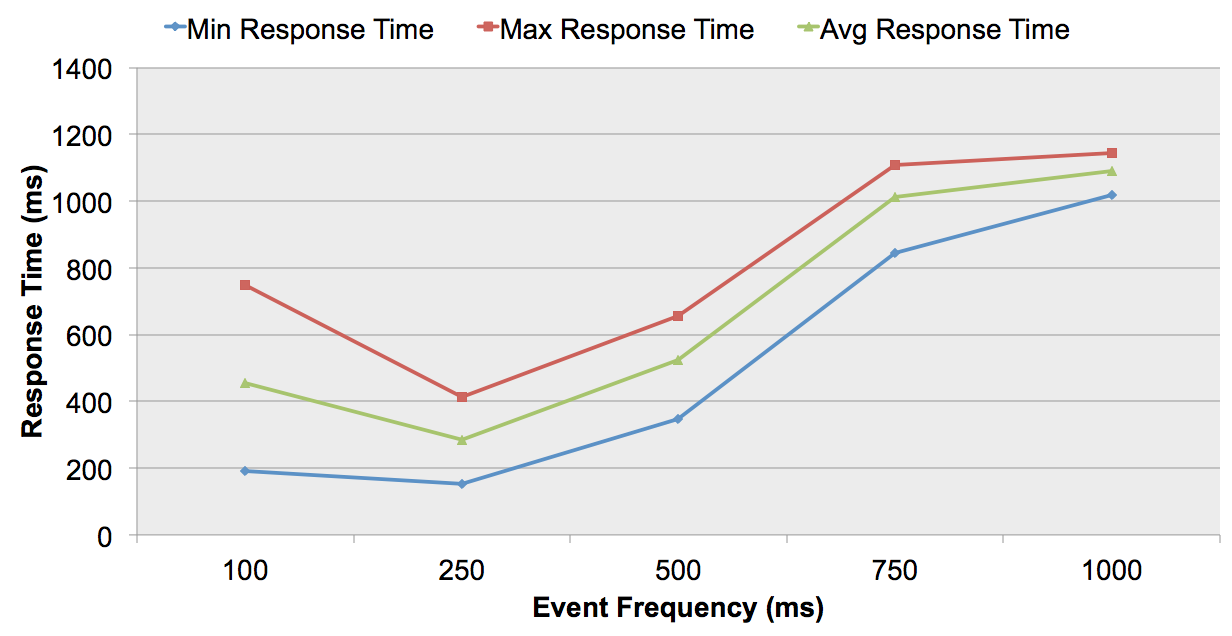
\includegraphics[width=90mm]{responseTime.png}
\caption{A simple caption}
\label{pic:responseTime}
\end{figure}
\paragraph{} To evaluate the effect of a large number of hosts generating frequent events, we analyzed response time versus event frequency. Figure 1 outlines our findings. We see that response time generally increases with event frequency (as the monitoring resolution is decreased to lower the event frequency). However, at the 10 events/sec mark, we see a large variance in response times due to increased processing overhead. Therefore, it is clear that there is a tradeoff between monitoring resolution and response times.

\paragraph{} Additionally, there was no significant difference between ping response times immediately before and after the host status update. For our experiments, we used the single switch topology described above on a virtualized Mininet network.

\section{Future Work}
\label{sec:future}

\paragraph{} Much work must be done to demonstrate the utility and performance of this kind of system, not the least of which is a performance comparison with HONE\cite{HONE}. Defining an extensible protocol for two-way communication between hosts and the controller will allow such a system to be leveraged by different kinds of applications (with different indicators of load). Currently, ‘spinning up’ new hosts simply involves changes to a data structure, but it is feasible to build a system that uses APIs (like those provided by Amazon’s EC2) to programmatically perform this task.

\subsection{Controller to Host Communication}

\paragraph{} Currently, SmartBalancer has only implemented one way communication from the end-hosts to the controller. Incorporating two way communications between the end-hosts and controllers would allow the controller to remotely control the end-hosts and perform functions such as enabling/disabling sending of specific events, limiting the number of events sent, and modifying key parameters that determine when the events are sent. This would greatly improve the flexibility of the system, and simplify system management.

\paragraph{} Host-to-host communication can potentially improve SmartBalancer’s scalability. While our current metrics do not require any aggregation, other metrics may require the controller to aggregate the data obtained from multiple hosts, which greatly increases burden on the controller. Delegating work to the end-hosts themselves would alleviate this increased overhead on the controller and allow the controller to handle more end-hosts.

\section{Conclusion}
\label{sec:conclusion}

\paragraph{} This work was intended to demonstrate that it is possible to build simple systems based on modern controller platforms that integrate information available at the host to make smarter decisions on network routing. We contend that we can build relatively simple appliances like load balancers without using controller platforms like HONE, which have complex measurement and querying mechanisms built specifically for host-integration.

\section{Acknowledgements}

\paragraph{} We would like to thank Joshua Reich for his help in structuring our Pyretic application. Also, we would like to thank Dr. Jennifer Rexford for making the world of SDN seem accessible, and for encouraging and refining our ideas on this project.

\bibliography{mybib}{}
\bibliographystyle{plain}

\end{document}







